% Drawing 76/01-2 -- folder 76, batch 01, archive page 11 (PDF page 12).
% Transcription: figure centrale : le même treillis dessiné plus grand, $D_{012}(F)$ en haut, $D_{02}(F)$, $D_{12}(F)$, puis $D_{01}$, $D_0$, $D_1$ et une case $\lbrace 1 \rbrace$ ; au-dessous une petite échelle encadrée « 2 3 4 5 ». À droite, un carré $D_{012} \to D_{12}$, $D_{02} \to D_2$, puis deux segments dessinés, l'un avec un point milieu, et « 23 ? »
% Kind: lattice of flags drawn larger; square; two segments. Method 2 (schematic redraw from the facsimile). Status: partial.
% Notes: Left: D012(F) on top, D02(F) and D12(F), then D01, D0, D1 and a small box (the transcription's "{1}", read here as a small boxed mark); arrows between node centres, schematised; below, the framed ladder "2 3 4 5". A vertical stroke separates the right part: the square D012 -> D12, D02 -> D2, and the two segments, one with a middle point, with "23 ?" below. The label D_I above is drawn.
% Coordinates: 1 unit = 1 mm = 1/100 of the crop width (bbox in page fractions: [0.35, 0.36, 0.88, 0.6]).
% Redrawn by Claude (claude-opus-5-5), issue #73, 2026-11-07; not checked by a human; not compiled (no TeX in the session).
% Rights: reproduces part of the work -- behind RENDER_TRANSCRIPTS, never published by itself.
\documentclass[tikz,border=3pt]{standalone}
\usepackage{amsmath,amssymb}
\usetikzlibrary{patterns,arrows.meta}
\tikzset{pencil/.style={black!45}, struck/.style={black!35}, mark/.style={circle,draw,inner sep=1.3pt}, pt/.style={circle,fill,inner sep=0.9pt}, opt/.style={circle,draw,fill=white,inner sep=1.1pt}}
\begin{document}
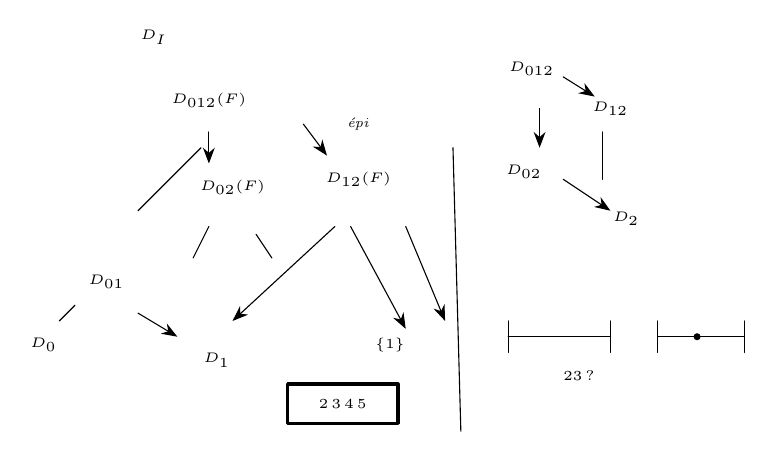
\begin{tikzpicture}[x=1mm,y=1mm,line cap=round,line join=round,font=\scriptsize]
\node[inner sep=1pt] at (23,-8) {\tiny $D_I$};
\node[inner sep=1pt] at (30,-16) {\tiny $D_{012}(F)$};
\node[inner sep=1pt] at (33,-27) {\tiny $D_{02}(F)$};
\node[inner sep=1pt] at (49,-26) {\tiny $D_{12}(F)$};
\node[inner sep=1pt] at (17,-39) {\tiny $D_{01}$};
\node[inner sep=1pt] at (9,-47) {\tiny $D_0$};
\node[inner sep=1pt] at (31,-49) {\tiny $D_1$};
\node[inner sep=1pt] at (53,-47) {\tiny $\{1\}$};
\draw[-{Stealth[length=2mm]}] (30,-20) -- (30,-24);
\draw[-{Stealth[length=2mm]}] (42,-19) -- (45,-23);
\node[inner sep=1pt] at (49,-19) {\tiny \textit{épi}};
\draw (29,-22) -- (21,-30);
\draw (30,-32) -- (28,-36);
\draw (36,-33) -- (38,-36);
\draw[-{Stealth[length=2mm]}] (21,-43) -- (26,-46);
\draw (13,-42) -- (11,-44);
\draw[-{Stealth[length=2mm]}] (46,-32) -- (33,-44);
\draw[-{Stealth[length=2mm]}] (48,-32) -- (55,-45);
\draw[-{Stealth[length=2mm]}] (55,-32) -- (60,-44);
\draw[very thick] (40,-52) -- (54,-52) -- (54,-57) -- (40,-57) -- cycle;
\node[inner sep=1pt] at (47,-54.5) {\tiny $2\,3\,4\,5$};
\draw (61,-22) -- (62,-58);
\node[inner sep=1pt] at (71,-12) {\tiny $D_{012}$};
\node[inner sep=1pt] at (81,-17) {\tiny $D_{12}$};
\node[inner sep=1pt] at (70,-25) {\tiny $D_{02}$};
\node[inner sep=1pt] at (83,-31) {\tiny $D_2$};
\draw[-{Stealth[length=2mm]}] (75,-13) -- (79,-15.5);
\draw[-{Stealth[length=2mm]}] (72,-17) -- (72,-22);
\draw[-{Stealth[length=2mm]}] (75,-26) -- (81,-30);
\draw (80,-20) -- (80,-26);
\draw (68,-46) -- (81,-46);
\draw (68,-44) -- (68,-48);
\draw (81,-44) -- (81,-48);
\draw (87,-46) -- (98,-46);
\draw (87,-44) -- (87,-48);
\draw (98,-44) -- (98,-48);
\node[pt] at (92,-46) {};
\node[inner sep=1pt] at (77,-51) {\tiny $23\,?$};
\end{tikzpicture}
\end{document}
